\documentclass[11pt, oneside]{article} 
\usepackage{geometry}
\geometry{letterpaper} 
\usepackage{graphicx}
	
\usepackage{amssymb}
\usepackage{amsmath}
\usepackage{parskip}
\usepackage{color}
\usepackage{hyperref}

\graphicspath{{/Users/telliott_admin/Dropbox/Tex/png/}}
% \begin{center} 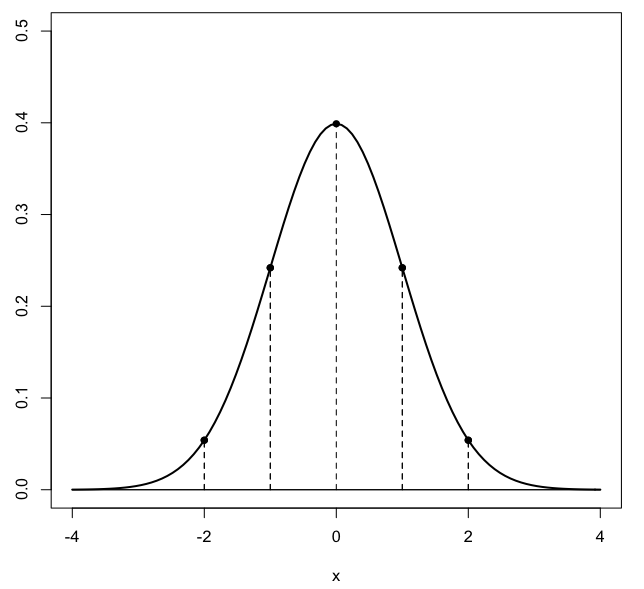
\includegraphics [scale=0.4] {gauss3.png} \end{center}

%break
\title{Snell's law}
\date{}

\begin{document}
\maketitle
\Large

\label{sec:Snells_law}

Consider the problem of a light ray passing from $P$ to $Q$, where $P$ is in air, and $Q$ is in a medium like water, with a higher refractive index and lower speed of light.  

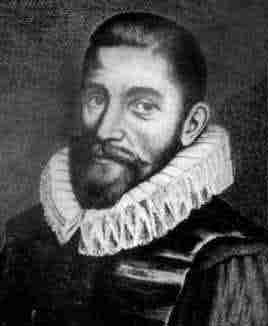
\includegraphics [scale=0.6] {Snell.jpg} 
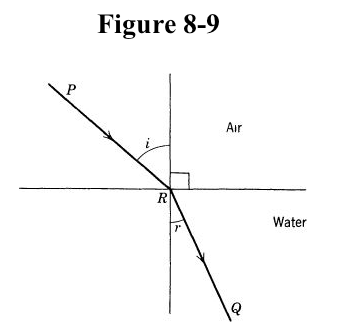
\includegraphics [scale=0.6] {snell_law.png}

The physical principle is that light takes the path of shortest time.  We need to find the $R$ that makes this true.

Suppose the total horizontal distance between $P$ and $Q$ is $d$.  Let $x$ be the horizontal distance from $P$ to $R$, then $d - x$ is the horizontal distance from $R$ to $Q$.  The vertical distances are fixed, let's call them $p$ (for $PR$) and $q$ (for $PQ$).

The time taken is the distance divided by the speed.  Let the speed of light in air be $u$ and the speed of light in water be $v$.  There are two segments of the trip:
\[ t_1 = \frac{\sqrt{x^2 + p^2}}{u} \]
\[ t_2 = \frac{\sqrt{(d-x)^2 + q^2}}{v} \]
\[ t = t_1 + t_2 = \frac{\sqrt{x^2 + p^2}}{u} + \frac{\sqrt{(d-x)^2 + q^2}}{v} \]

We have time $t$ as a function of $x$ and we take the first derivative and set it equal to zero:

\[ \frac{x}{u \sqrt{x^2 + p^2}} + \frac{-(d-x)}{v \sqrt{(d-x)^2 + q^2}}  = 0  \]
\[ \frac{x}{u \sqrt{x^2 + p^2}} = \frac{(d-x)}{v \sqrt{(d-x)^2 + q^2}}  \]

Rather than fool with the square roots, notice that
\[ \sqrt{x^2 + p^2} = PR \]
and
\[ \sqrt{(d-x)^2 + q^2} = RQ \]
so
\[ \frac{x}{u \sqrt{x^2 + p^2}} = \frac{(d-x)}{v \sqrt{(d-x)^2 + q^2}}  \]
becomes
\[ \frac{x}{u \ {PR}} = \frac{(d-x)}{v\  {RQ}}  \]

Furthermore $x/PR = \sin \theta_i$ and $(d-x)/RQ = \sin \theta_r$ so
\[ \frac{\sin \theta_i}{u} = \frac{\sin \theta_r}{v}  \]
The sines of the angles for each side of the barrier are in the same ratio as the velocities in the respective medium.
\[ \frac{\sin \theta_i}{\sin \theta_r} = \frac{u}{v}  \]
\[ \sin \theta_r = \frac{v}{u} \ \sin \theta_i \]

Since the speed of light in air is higher than in water $u > v$, $v/u < 1$ which means that $\sin \theta_r < \sin \theta_i$ and thus $\theta_r < \theta_i$.

We can also use the refractive index $n$ which is proportional to the reciprocal of the speed.
\[ \frac{\sin \theta_i}{\sin \theta_r} = \frac{n_r}{n_i}  \]

\end{document}